\documentclass[a4paper]{article}
\usepackage[utf8]{inputenc}
\usepackage{cite}
\usepackage[T1]{fontenc}

%% Sets page size and margins
\usepackage[a4paper,top=3cm,bottom=2cm,left=3cm,right=3cm,marginparwidth=1.75cm]{geometry}

%% Useful packages
\usepackage{amsmath}
\usepackage{floatrow}
\usepackage{graphicx}
\graphicspath{ {./images/} }
\usepackage[colorinlistoftodos]{todonotes}
\usepackage[colorlinks=true, allcolors=blue]{hyperref}
\usepackage{amsmath}
\usepackage{chngcntr}
\usepackage{wrapfig}
\usepackage{caption}
\usepackage{subcaption}
\usepackage{listings}
\usepackage{placeins}
\usepackage{multicol}

\usepackage{csvsimple}
\usepackage{xcolor}
\usepackage{listings}

\usepackage[spanish]{babel}
\selectlanguage{spanish}

\renewcommand{\lstlistingname}{Código}% 
\renewcommand{\lstlistlistingname}{Lista de código}% List of Listings -> List of Algorithms

% extracted from internet: https://timmurphy.org/2014/01/27/displaying-code-in-latex-documents/
\definecolor{lbcolor}{rgb}{0.93,0.93,0.93}
\lstset{  
    frame=tb, % draw a frame at the top and bottom of the code block
    tabsize=4, % tab space width
    showstringspaces=false, % don't mark spaces in strings
    numbers=left, % display line numbers on the left
    commentstyle=\color{green}, % comment color
    keywordstyle=\color{blue}, % keyword color
    stringstyle=\color{red},
    backgroundcolor=\color{lbcolor}
}
%sdf
\definecolor{main-color}{rgb}{0.6627, 0.7176, 0.7764}
\definecolor{back-color}{rgb}{0.1686, 0.1686, 0.1686}
\definecolor{string-color}{rgb}{0.3333, 0.5254, 0.345}
\definecolor{key-color}{rgb}{0.8, 0.47, 0.196}
\lstdefinestyle{idlstyle}
{
    language = C++,
    keywordstyle = {\color{key-color}},
    keywordstyle = [3]{\color{blue}},
    otherkeywords = {in, int ,interface, out, inout},
    morekeywords = [3]{in, out, inout}
}

\setcounter{secnumdepth}{3}
\setcounter{tocdepth}{3}

% \title{Integrating COMPSs and OmpSs Programming Models to support distributed heterogeneous computing environments}
\title{Integrating COMPSs and OmpSs Programming Models to support distributed heterogeneous computing environments}
\author{Marc Domínguez de la Rocha}
\date{Febrero 2019}

\begin{document}

\maketitle

\newpage
\renewcommand{\contentsname}{Índice}
\tableofcontents
\newpage


% La siguiente seccion enmarca el contexto
% que envuelve al proyecto y de alguna
% manera el por qué
\section{Contexto}

Hoy en día se tiende a tener distintos recursos de cómputo en un solo dispositivo, por ejemplo, en un teléfono móvil ya tenemos al menos un procesador y una tarjeta gráfica, pero no tan sólo en el ámbito más mundano (aunque no nos demos cuenta), si no que en los más profesionales y especializados está siendo también cada vez más común la heterogeneidad de los recursos de computación. 
\par\bigskip

El proyecto pretende facilitar la gestión de estos recursos de computación en entornos distribuidos, brindando un método robusto y eficiente para programar aplicaciones en estos entornos.
%Quienes son los actores? Quien se beneficia?


\subsection{Introducción}

Este proyecto es un Trabajo de Fin de Grado del Grado en Ingeniería Informática, especializado en el área de Ingeniería de Computadores. El grado es impartido por la \textit{Facultat d'Informàtica de Barcelona (FIB)} centro perteneciente a la \textit{Universitat Politècnica de Catalunya (UPC)}. 
\par\bigskip

El proyecto se desarrollará conjuntamente con el \textit{Barcelona Supercomputing Center (BSC)}, estudiaremos como podemos integrar los modelos de programación \textit{COMPSs} y \textit{OmpSs} para alcanzar este objetivo, implementaremos un prototipo y evaluaremos su rendimiento y características deseadas. 
%Indagar en cuales son estas caracteristicas? 

\subsection{Actores}

Los actores en este proyecto serán las personas que tomen parte en él, ya sea de manera directa o indirecta. Con esto quiero decir, que tanto las personas que tomen parte en el desarrollo \textit{per se} como las personas que se nutran de este, serán los actores.

\begin{itemize}
 \item \textbf{Desarrollador:} La figura del desarrollador \textbf{debe} ser la persona que trabaje de manera más directa en el proyecto. En este proyecto únicamente habrá un desarrollador que ha elaborado la documentación que leerás a continuación y dará forma a los objetivos tangibles del proyecto.  
 \item \textbf{Director y codirector:} Pese a que el desarrollador tendrá el papel principal en el proyecto, el director y el codirector le guiarán en el camino abierto que es el desarrollo del proyecto. Se establecerán reuniones de seguimiento donde serán capaces de hacer un correcto supervisamiento de las actividades propuestas para el proyecto.
 \item \textbf{Barcelona Supercomputing Center:} De manera directa el centro otorga al desarrollador un lugar de trabajo y un equipo informático. Por otra parte, cuenta con el soporte por parte de los equipos de desarrollo de \textit{COMPSs} (del cual forma parte el desarrollador) y de \textit{OmpSs} para cualquier incidencia relacionada con su \textit{software} y derivados.
 \item \textbf{Beneficiarios:} \todo{Por determinar}%TODO Quienes son?
 
\end{itemize}

\section{Estado del arte}

%check si te estas patillando lo de ``centenares''
Existen centenares de modelos de programación, véanse \textit{OpenMP}, \textit{OmpSs}, \textit{COMPSs} y un largo etcétera. De alguna manera el objetivo en común fue y es aprovechar los cada vez más abundantes recursos en las máquinas, que finalmente no sólo han crecido en abundancia si no en diversidad. La filosofía sigue siendo la misma, sacar el mayor rendimiento posible a nuestras máquinas. \par\bigskip

Para esto son necesarios modelos de programación que nos den la posibilidad de utilizar los recursos y nos ayuden a explotar la posible sinergia entre estos en ciertas aplicaciones. 
\par\bigskip
La integración de los modelos propuestos \textit{COMPSs} y \textit{OmpSs} nos otorgará esta posibilidad de utilizar todos los recursos de la máquina, a continuación se ahonda en las características de ambos.

\subsection{COMPSs}

\textit{COMPSs} es desarrollado por el grupo \textit{WDS - Workflows and Distributed Computing} que pertenece al departamento de \textit{CS - Computer Science}.
\par\bigskip

\textit{COMPSs} es un modelo de programación para entornos distribuidos\cite{badia2015comp}, dado que se basa en la generación de tareas por parte de un programa principal ejecutado en secuencial que llamaremos \textit{master}, mediante simples modificaciones del código podemos conseguir que este se ejecute de manera distribuida. A los procesos que ejecutarán las tareas generadas por el \textit{master} los llamaremos \textit{workers}.  \par\bigskip

Para facilitar más aún el uso del modelo, está dotado de un sistema de \textit{runtime}, que tal y como indica la palabra coexiste con la aplicación. Este sistema de \textit{runtime} se encarga de detectar las dependencias que puedan surgir entre las tareas que genera el \textit{master} y las ejecuta a medida que las dependencias se resuelven. 
%\par\bigskip

\subsubsection{Modelo de programación}

El \textit{runtime} de \textit{COMPSs} está implementado en \textit{Java} por lo cuál se soporta dicho lenguaje, además se desarrollaron los \textit{bindings} de \textit{Python} y \textit{C/C++} para facilitar el portaje de aplicaciones en estos lenguajes a \textit{COMPSs}. 
\par\bigskip

Dicho esto, centraremos nuestros esfuerzos en \textit{C} y \textit{C++}. Para desarrollar una aplicación de \textit{COMPSs} en \textit{C/C++} necesitamos el código que ejecutará el \textit{master} (recordemos, en secuencial), una interfaz que especificará las funciones que ejecutadas en el \textit{master}, \textit{a posteriori} serán ejecutadas en los \textit{workers}, y el código que realmente implementan estas tareas. 
\par\bigskip

Veamos en orden de enumeración ejemplos de los componentes de una aplicación.

\begin{lstlisting}[caption={Interfaz de la aplicación 'ejemplo'.},captionpos=b, label={lst:ejemplo.idl}, style=idlstyle]
interface ejemplo {
    void funcionEjemplo(in int a, out int[a] array_a);
};
\end{lstlisting}

La interfaz de la imagen superior define una función llamada funcionEjemplo con un parámetro de entrada y uno de salida, las palabras clave \textit{in} y \textit{out} respectivamente otorgan estas propiedades a los parámetros, también se puede combinar con \textit{inout}. \smallskip

\begin{lstlisting}[caption={Fracción del código del \textit{master}}, captionpos=b, label={lst:ejemplo.cc}, language=C++]
    compss_on();

    int a = 10;
    int* array_a;

    funcionEjemplo(a, array_a);

    compss_wait_on(array_a);

    compss_off();
\end{lstlisting}

Esta imagen muestra el código del \textit{master} de manera reducida. Es tan sencillo como prometía, encendemos el \textit{runtime} de \textit{COMPSs}, preparamos los parámetros de la función, esperamos a los parámetros de salida y apagamos el \textit{runtime}. 

\begin{figure}[H]
    \centering
    \caption{Proceso de compilado de una aplicación COMPSs C/C++}
%    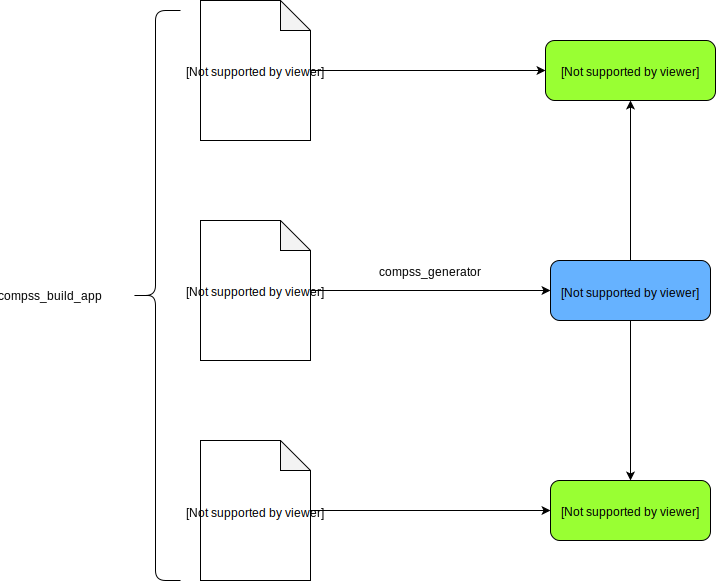
\includegraphics[width=\textwidth]{proceso_compilado.jpg}
    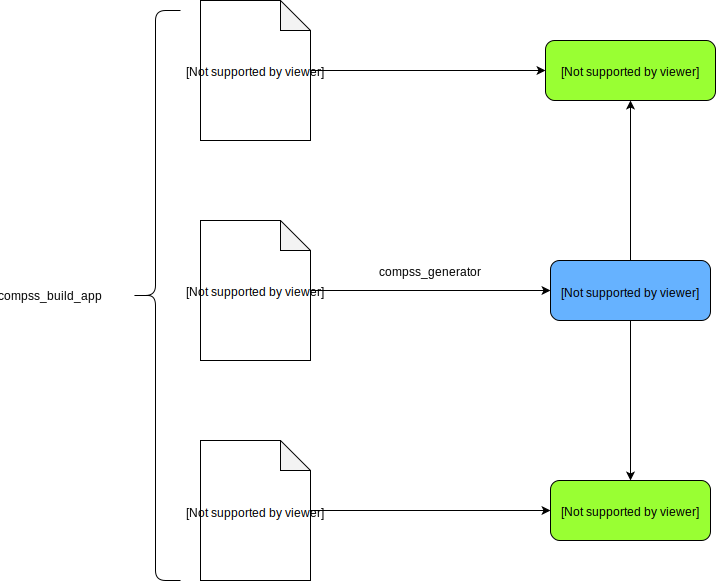
\includegraphics[scale=0.5]{proceso_compilado.jpg}
    \label{fig:proceso_compilado}
\end{figure}


\subsection{OmpSs}

\textit{OmpSs} es desarrollado por el grupo \textit{PM - Programming Models}, perteneciente también al departamento de \textit{CS - Computer Science}.
\par\bigskip

\textit{OmpSs} es un modelo de programación que intenta explotar el paralelismo de las aplicaciones de una manera sencilla y aprovechando al máximo los recursos de la máquina. 
\par\bigskip
El nombre del modelo proviene de \textit{OpenMP} y \textit{StarSs} (modelo que desarrolló el \textit{BSC}), este integra funcionalidades presentes en ambos. Por parte de \textit{OpenMP} se quiere tomar la facilidad de paralelizar una aplicación secuencial insertando pragmas, y de \textit{StarSs} el modelo de ejecución basado en un \textit{thread-pool} y que permite la ejecución de código en más recursos que el procesador, es decir, que ofrece fácil gestión de recursos heterogéneos.

\subsection{COMPSs+OmpSs}


\bibliography{bibliography}{}
\bibliographystyle{plain}
\end{document}
